\section{基礎資料型態型別}
\subsection{儲存資料}
電腦是以二進位儲存資料,二進位是指數字是由 $0,1$ 組成,相較於常見的十進位是由 $0~9$ 組成,一個 $0$ 或 $1$ 稱為位元 (bit),8 bits 稱為 byte(位元組),byte 是電腦基本儲存單位,下表為各種常見電腦儲存單位。\\
\begin{tabular}{|r|l|} \hline 1B & 1 byte \\\hline 1KB & 1024 bytes \\\hline 1MB & 1024 KBs \\\hline 1GB & 1024 MBs\\\hline \end{tabular}\\
在 C/C++ 裡,將所有的基礎資料型態分成四類說明,依序是整數、浮點數、字元、布林值。
\subsection{整數}
整數分成兩個部分,最左邊的位元表示正負號(0:正,1:負),其餘表示數字。\\
通常會以 int 作為整數型態,int 兼顧範圍大小和記憶體大小。如果存的數字保證不會用到負數的話,可以在前面加上 unsigned,這樣最左邊的位元也會用來表示數字。
\subsubsection{溢位}
上表有給出每種型態的範圍。假設兩個相同型態加總後超過範圍,那麼最高位(最左邊)進位後會被捨去,造成結果和正確值不同,這個狀況稱之為溢位。
\lstinputlisting{Type/overflow.cpp}
% TODO:溢位範例圖
\begin{tabular}{|r|l|l|l|} \hline 名稱 & 別稱 & 位元組 & 範圍 \\\hline short & short int, signed short int & 2 & –32,768 to 32,767 \\\hline unsigned short & unsigned short int & 2 & 0 to 65,535 \\\hline int & signed, signed int & 4 & –2,147,483,648 to 2,147,483,647 \\\hline unsigned int & unsigned & 4 & 0 to 4,294,967,295 \\\hline long long & long long int, signed long long & 8 & –9,223,372,036,854,775,808 to 9,223,372,036,854,775,807 \\\hline unsigned long long & unsigned long long int & 8 & 0 to 18,446,744,073,709,551,615 \\\hline \end{tabular}\\
\subsection{浮點數}
浮點數分成 3 個部分,sign bit(符號):用來表示正負號、exponent(指數):用來表示次方數、mantissa(尾數):用來表示精確度。\\
\begin{figure}
  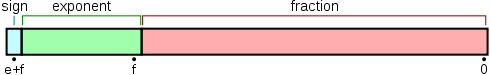
\includegraphics[]{Type/IEEE754.png}
  \caption{ASCII from Wiki}
  \label{fig:IEEE754}
\end{figure}\\
\begin{tabular}{|r|l|l|l|l|} \hline 名稱 & 別稱 & 位元組 & 範圍 & 精度 \\\hline float & 無 & 4 & 3.4E +/- 38 & 7 digits \\\hline double & long double & 8 & 	1.7E +/- 308 & 15 digits \\\hline \end{tabular}\\
\subsubsection{浮點數誤差}
浮點數儲存也會有限制,如果小數點後個位數過多,會被捨去造成誤差,float 保證以 10 進位表示時,小數點後 7 位內會是正確,double 則是 15 位。
\lstinputlisting{Type/floatError.cpp}
% TODO:浮點數範例圖
\subsection{字元}
C/C++ 採用 ASCII 字元集,一個數字對應一個字母,但這份字元集只有英文字母、數字、常見的符號,其他國家的文字則無。\\
\begin{tabular}{|r|l|l|l|} \hline 名稱 & 別稱 & 位元組 & 範圍\\\hline char & 無 & 1 & -128 to 127 \\\hline unsigned char & 無 & 1 & 0 to 255 \\\hline wchar & 無 & 2 & 0 to 65,535 \\\hline\end{tabular}\\
\begin{figure}
  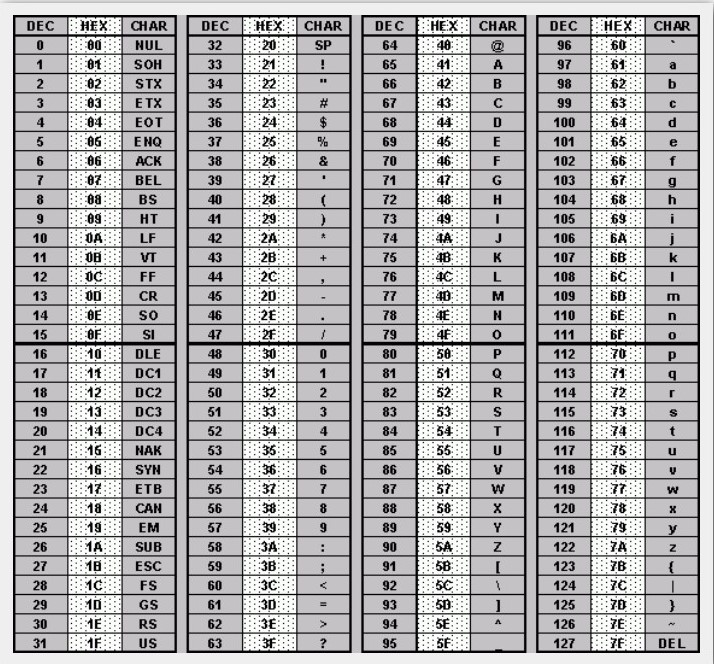
\includegraphics[]{Type/ASCII.jpg}
  \caption{ASCII from http://www.thedawncreative.com/}
  \label{fig:ASCII}
\end{figure}
\subsection{布林值(C++)}
布林值只有兩種植 Ture(1 或是說 非 0)、False(0),當作邏輯變數,相較利用整數型態,有兩個有優勢,一個是節省記憶體,二是可以明確表示是用來記錄 True/False 狀態。\\
\begin{tabular}{|r|l|l|l|} \hline 名稱 & 別稱 & 位元組 & 範圍\\\hline bool & 無 & 1 & 0 to 1 \\\hline\end{tabular}\\
\subsection{後記}
還有一個型態 enum,這裡先不提。\\
\begin{tabular}{|r|l|l|l|} \hline 名稱 & 別稱 & 位元組 & 範圍\\\hline enum & 無 & varies & TBA \\\hline\end{tabular}\\
